\documentclass{beamer}


\mode<presentation>
{
  \usetheme{CambridgeUS}
	\usecolortheme{beaver}
  % or ...

  \setbeamercovered{transparent}
  % or whatever (possibly just delete it)
}


\usepackage{xeCJK}
\usepackage[english]{babel}
\usepackage[utf8]{inputenc}
\usepackage{times}
\usepackage[T1]{fontenc}
\usepackage{hyperref}
\usepackage{pifont}
\usepackage{bibentry}
\usepackage{verbatim}
\newcommand{\cmark}{\ding{51}}%
\newcommand{\xmark}{\ding{55}}%
\setCJKmainfont{WenQuanYi Micro Hei}


\title[开源软件基础] 
{开源软件基础}
\subtitle{数据获取案例}

\author[Zhilei Ren] 
{Zhilei Ren}

\institute[OSCAR Team] % (optional, but mostly needed)
{
\\
\includegraphics[width=0.2\textwidth]{../../utils/logo.jpg}\\
OSCAR Team, School of Software, 
Dalian University of Technology
}


\subject{Open source software}



\pgfdeclareimage[height=0.5cm]{university-logo}{../../utils/logo.jpg}
\logo{\pgfuseimage{university-logo}}



% Delete this, if you do not want the table of contents to pop up at
% the beginning of each subsection:
\AtBeginSubsection[]
{
  \begin{frame}<beamer>{Outline}
    \tableofcontents[currentsection,currentsubsection]
  \end{frame}
}


% If you wish to uncover everything in a step-wise fashion, uncomment
% the following command: 

%\beamerdefaultoverlayspecification{<+->}

\setbeamertemplate{section in toc}[circle]
\setbeamertemplate{items}[circle]
\setbeamertemplate{caption}[numbered]
\setbeamertemplate{bibliography item}{\insertbiblabel}
\setbeamertemplate{bibliography entry title}{}
\setbeamertemplate{bibliography entry journal}{}

\begin{document}

\begin{frame}
  \titlepage
\end{frame}

%\begin{frame}{Outline}
%  \tableofcontents[currentsection,currentsubsection, 
%    hideothersubsections, 
%    sectionstyle=show,
%]
%\end{frame}

\AtBeginSection[]
{
 \begin{frame}<beamer>
 \frametitle{Outline}
 \tableofcontents[currentsection]
 \end{frame}
}
\section{简单案例} % (fold)
\label{sec:简单案例}

% section 简单案例 (end)

\section{Hacker News} % (fold)
\label{sec:Hacker News}
\begin{frame}[t]{Paul Graham}
    \begin{minipage}
        {0.6\linewidth}
        保罗·格雷厄姆（Paul Graham，1964年－），美国著名程序员、风险投资家、博客和技术作家。他以Lisp方面的工作而知名，也是最早的Web应用Viaweb的创办者之一，后来以近5千万美元价格被雅虎收购，成为Yahoo! Store。他的著作包括《On Lisp》（1993），《ANSI Common Lisp》（1995）和《Hackers \& Painters》（2004）
    \end{minipage}
    \begin{minipage}
        {0.35\linewidth}
    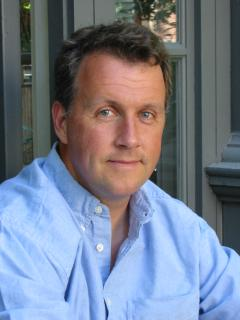
\includegraphics[width=0.8\linewidth]{paul.jpg}
    \end{minipage}
\end{frame}
\begin{frame}[t]{今天就能开始用的小知识}
    \centering
    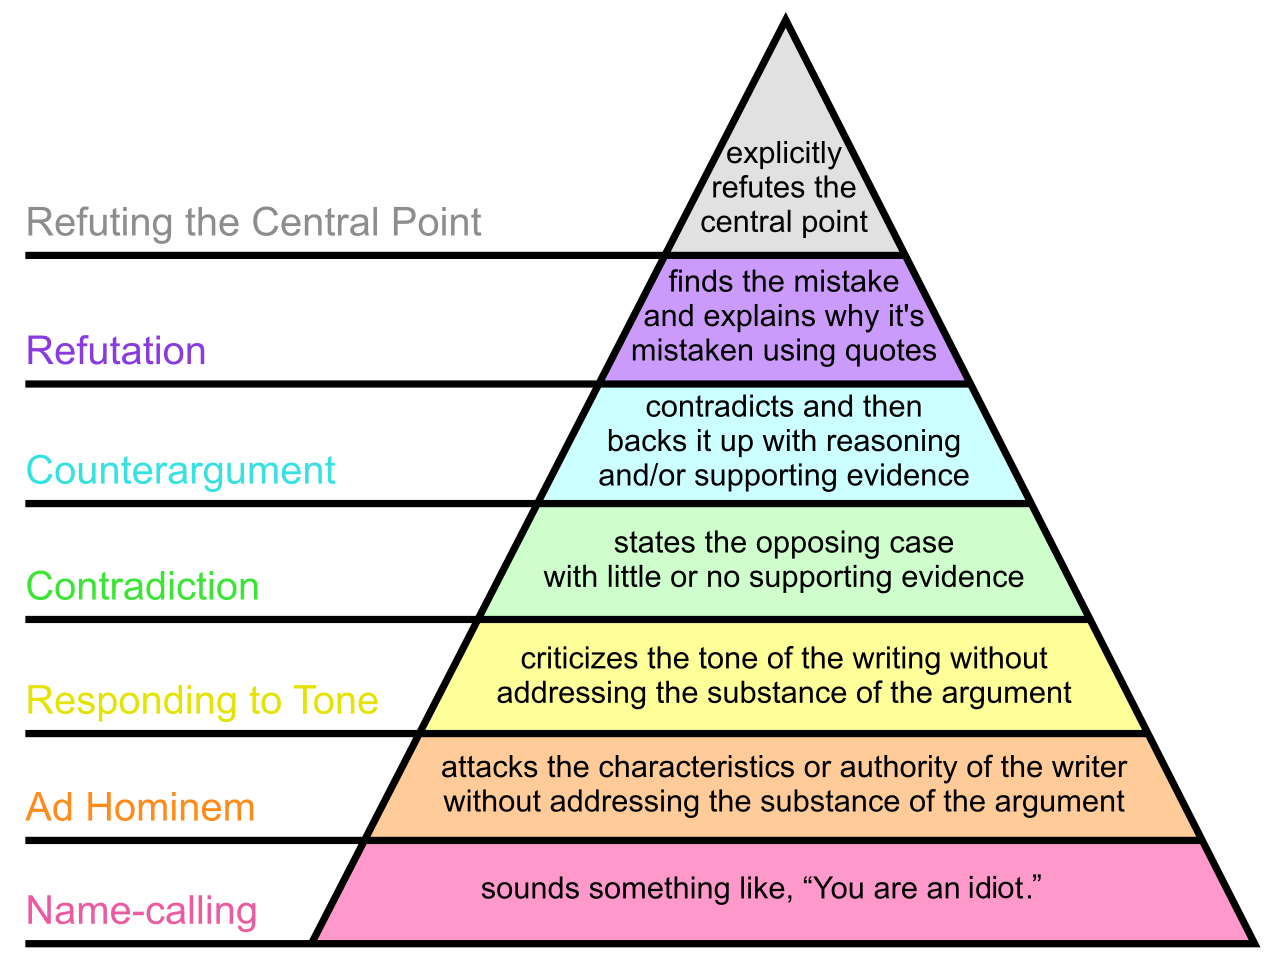
\includegraphics[width=0.6\linewidth]{hierarchy-disagreement.png}

    Hierarchy of disagreement\footnote{\url{http://www.paulgraham.com/disagree.html}}\footnote{\url{http://money.163.com/15/0211/17/AI6JHSTJ00253G87.html}}
\end{frame}

\begin{frame}[t]{书籍推荐}
    \begin{minipage}
        {0.45\linewidth}
        
\includegraphics[width=0.8\linewidth]{hacker.jpg}
    \end{minipage}
    \begin{minipage}
        {0.45\linewidth}
        \begin{block}
            {黑客与画家}
            Hackers \& Painters: Big Ideas from the Computer Age is a collection of essays from Paul Graham discussing hacking, programming languages, start-up companies, and many other technological issues.

            "Hackers \& Painters" is also the title of one of those essays.
        \end{block}
    \end{minipage}


\end{frame}
\begin{frame}[t]{Hacker News\footnote{\url{https://en.wikipedia.org/wiki/Hacker_News}}}
    \begin{minipage}
        {0.45\linewidth}
        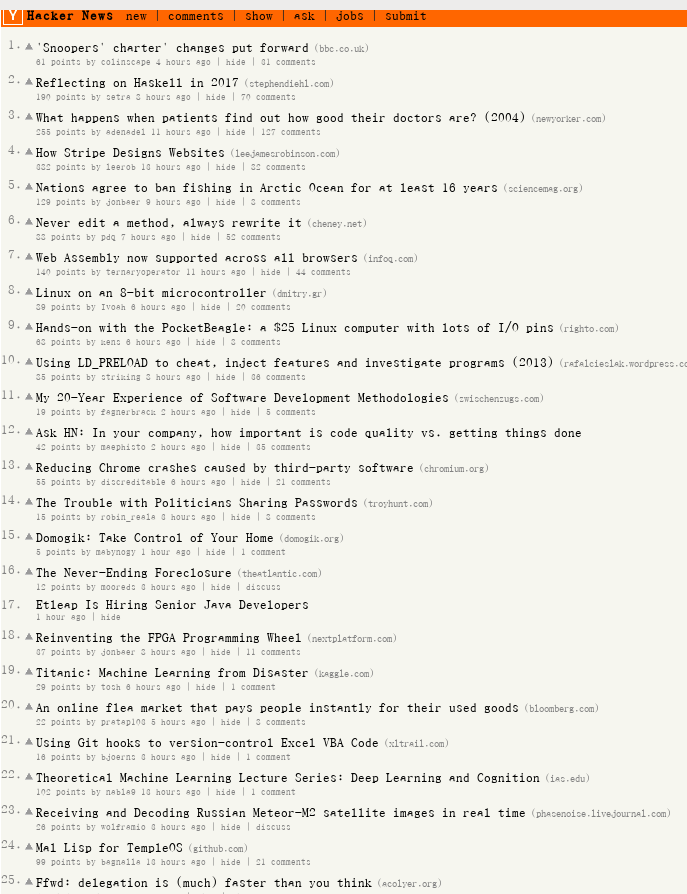
\includegraphics[width=0.9\linewidth]{hacker-news.png}
    \end{minipage}
    \begin{minipage}
        {0.45\linewidth}
        \begin{block}
            {Hacker News}
    Hacker News is a social news website focusing on computer science and entrepreneurship. It is run by Paul Graham's investment fund and startup incubator, Y Combinator. In general, content that can be submitted is defined as "anything that gratifies one's intellectual curiosity". 
        \end{block}
    \end{minipage}

\end{frame}
\begin{frame}[t,fragile]{Program skeleton}
\begin{verbatim}
url = "http://oscar-lab.org/puzzle.html"
txt = requests.get(url).text
soup = bs4.BeatifulSoup(txt, "lxml")
tbody = soup.find("tbody")
for tr in tbody.find_all("tr"):
    for td in tr.find_all("td"):
        #traverse all cells

\end{verbatim}
\end{frame}
% section Hacker News (end)

\section{Linux Kernel Mailing List} % (fold)
\label{sec:Linux Kernel Mailing List}
\begin{frame}[t]{Linux Kernel Mailing List\footnote{\url{https://lkml.org/}}}
    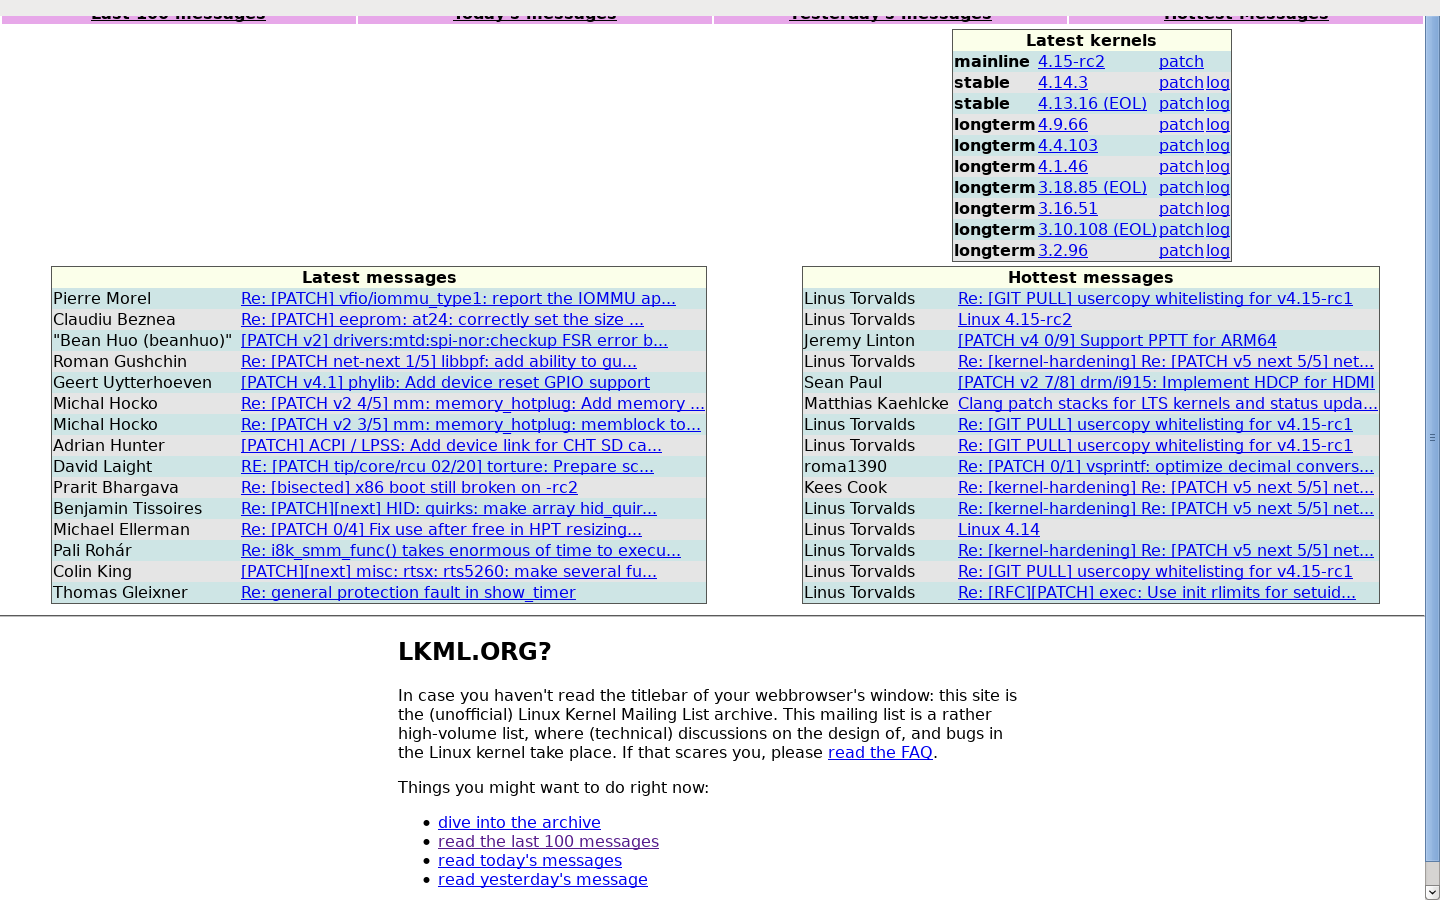
\includegraphics[width=0.9\linewidth]{lkml.png}
\end{frame}

\begin{frame}[t]{Linux Kernel Mailing List}
    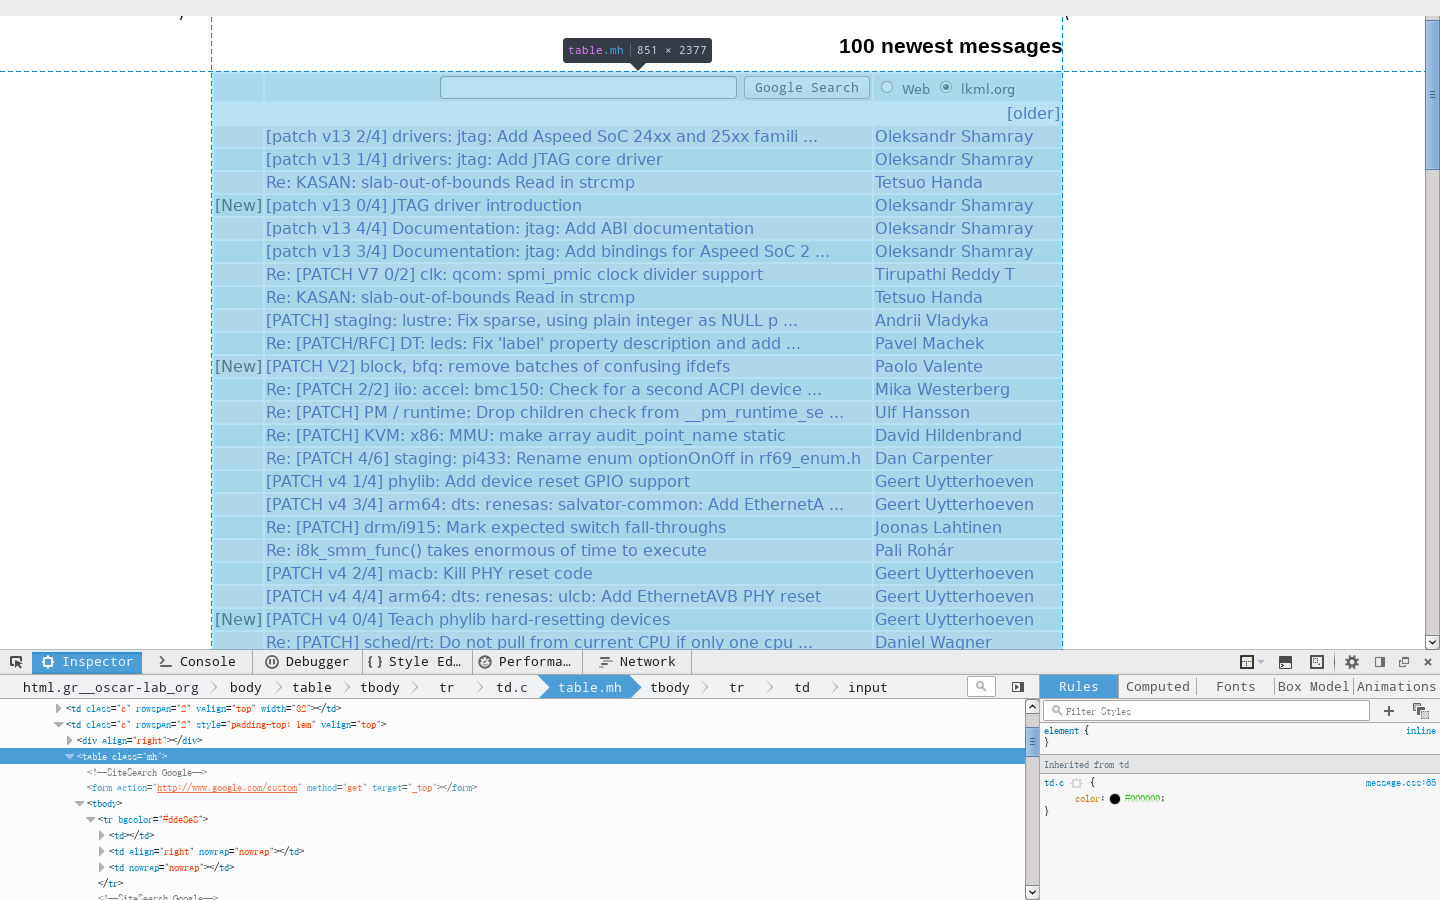
\includegraphics[width=0.9\linewidth]{inspect.png} 
\end{frame}

% section Linux Kernel Mailing List (end)

\section{Slides Generator} % (fold)
\label{sec:Slides Generator}
\begin{frame}[t]{Slidesgen}
    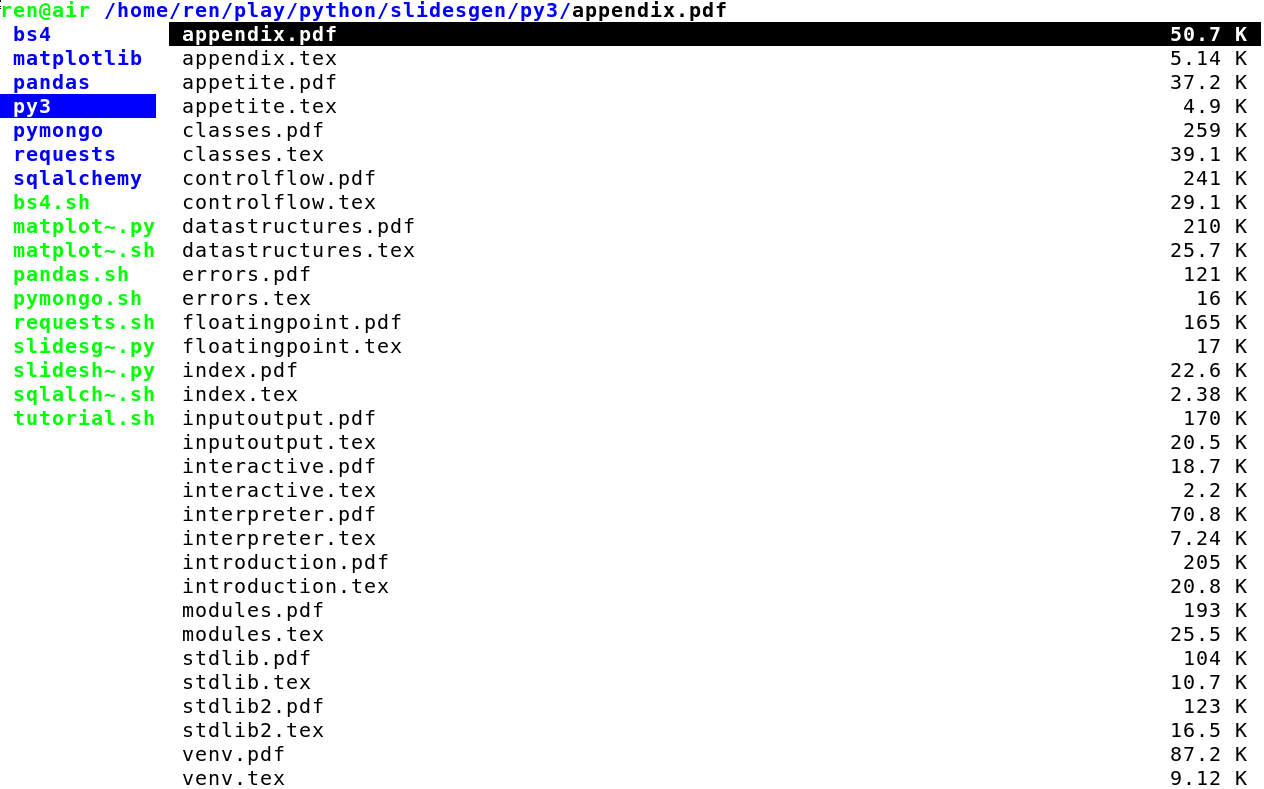
\includegraphics[width=0.9\linewidth]{slidesgen.png}
    
\end{frame}

\begin{frame}[t,fragile]{Program skeleton}
    \tiny
    \begin{verbatim}
txt = requests.get(URL).text
doc = bs4.BeautifulSoup(txt, "lxml")
title = doc.find('title').text
current_frame_title = title
interested = doc.find_all(['h1', 'h2', 'pre', 'p'])
for node in interested:
    if node.name == 'h1':
        #处理h1
    elif node.name == 'h2':
        #处理h2
    elif node.name == 'p':
        #处理p
    elif node.name == 'pre':
        #处理pre
    else:
        #处理异常
\end{verbatim}
\end{frame}

% section Slides Generator (end)

\end{document}
